% Shows the results of running our Method in the setting described in the Experimental Setup section.
% Includes reasonable comparisons and ablations so that all the claims we made in the Abstract and Intro are justified.

% The purpose of this section is to check the contributions of the paper.
% Not to introduce new ideas. No new methods or datasets should be introduced here (put it in the Methods and Experimental Setup sections).
% From the Methods and Experimental Setup section, readers should basically be able to guess exactly the experiments you're going to run.

% MAIN CHART with killer caption (ideally this caption explains the whole paper)
% [PARAGRAPH EXPLAINING MAIN CHART]


\begin{figure}[h]
    \centering
    \begin{minipage}{0.3\linewidth}
        \centering
        % If you want to frame the image, uncomment the next line and comment out the original \includegraphics line
        % \fbox{\includegraphics[width=\linewidth]{figs/figure.png}}
        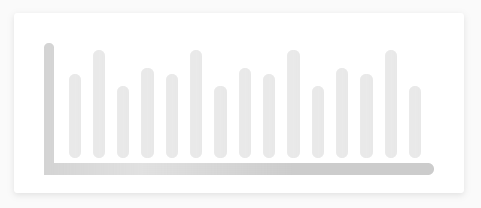
\includegraphics[width=\linewidth]{assets/chart_placeholder.png}
    \end{minipage}
    \caption{Figure clearly showing technical details of measurements made by experiments.}
    \label{fig:system}
    \end{figure}

% A set of experiments that usefully explore how good/interesting the method/model/central investigation of the paper is, and which tell a clear and cohesive story.
% Everything that appears in the Methods/Experimental Setup section should be tested, with ablations if feasible.

% We want to show absolute performance, performance relative to baselines and previous methods
% and performance compared to other methods introduced in this work and/or ablations.

% [CORE TABLE]
% Use booktabs style for all tables

\begin{table}[ht]
    \centering
    \begin{tabular}{lcccc}
        \hline
        Method & Metric 1 & Metric 2  & Metric 3 \\
        \hline
        Baseline 1 [CITE] & 0.013 & 3.2 & \textbf{0.999} \\
        Baseline 2 [CITE] & 0.034 & 3.4 & 0.995 \\
        Method 1 (ours) & \textbf{0.011} & 3.8 & 0.999 \\
        Method 2 (ours) & 0.012 & 3.6 & 0.999 \\
    \end{tabular}
    \caption{Enter caption here!}
    \label{table:core_table}
\end{table}

% [PARAGRAPH EXPLAINING TABLE]


% SUPPORTING CHARTS
% [PARAGRAPH EXPLAINING SUPPORTING CHARTS]

% Each table/chart should show the results of a single experiment.
% Try to go for at least one chart and one table here.
% For additional results (either here or the appendix),
% prefer charts to tables when it's unclear which to choose.

% Where possible include error bars on charts and confidence intervals in tables.
